%%%%%%%%%%%%%%%%%%%%%%%%%%%%%%%%%%%%%%%%%%%%%%%%%%%%%%%%%%%
% --------------------------------------------------------
% Tau
% LaTeX Template
% Version 2.4.0 (14/05/2024)
%
% Author: 
% Guillermo Jimenez (memo.notess1@gmail.com)
% 
% License:
% Creative Commons CC BY 4.0
% --------------------------------------------------------
%%%%%%%%%%%%%%%%%%%%%%%%%%%%%%%%%%%%%%%%%%%%%%%%%%%%%%%%%%%
% --------------------------------------------------------
%			  RECOMMENDATION FOR SPANISH BABEL
% --------------------------------------------------------
% \usepackage[spanish,es-nodecimaldot,es-noindentfirst]{babel}
% --------------------------------------------------------
%%%%%%%%%%%%%%%%%%%%%%%%%%%%%%%%%%%%%%%%%%%%%%%%%%%%%%%%%%%

\documentclass[9pt,a4paper,twoside]{tau}
\usepackage[english]{babel}
\usepackage{tauenvs}

%----------------------------------------------------------
% TITLE
%----------------------------------------------------------

\title{Writing an academic article or lab report with tau \LaTeX\ class}

%----------------------------------------------------------
% AUTHORS, AFFILIATIONS AND PROFESSOR
%----------------------------------------------------------

\author[a,1]{Author One}
\author[b,2]{Author Two}
\author[b,c,3]{Author Three}

%----------------------------------------------------------

\affil[a]{Affiliation of author one}
\affil[b]{Affiliation of author two}
\affil[c]{Affiliation of author three}

\professor{Professor/Authority or other information}

%----------------------------------------------------------
% FOOTER INFORMATION
%----------------------------------------------------------

\institution{College name}
\footinfo{\LaTeX\ Template}
\theday{May 14, 2024}
\etal{Author last name et al.}
\course{Creative Commons CC BY 4.0}

%----------------------------------------------------------
% ABSTRACT AND KEYWORDS
%----------------------------------------------------------

\begin{abstract}    
    Welcome to tau ($\tau$) \LaTeX\ class for making academic articles and lab reports. In this example template, we will guide you through the process of using and customizing this class to your needs. For more information of this class check out the appendix section. There, you will find codes that define key aspects of the template, allowing you to explore and modify them.
\end{abstract}

%----------------------------------------------------------

\keywords{\LaTeX\ class, lab report, academic article, tau class}

%----------------------------------------------------------

\begin{document}
		
    \maketitle\thispagestyle{firststyle}\tauabstract
    \tableofcontents

%----------------------------------------------------------

\section{Introduction}

    \taustart{W}elcome to \textit{tau class} template for preparing your academic article or lab report. In this guide, we will take a look at its main features and how you can customize some aspects to this class. Due to its clean and structured code, users can easily customize this class to their specific needs and preferences. In addition, this template uses an easy-to-read and high quality font with \textit{stix2}. Notable features include custom colors, environments and settings for including code from Matlab, C, C++ and \LaTeX.
    
\section{Document styling}

    \subsection{Title}
	
        The \verb*|\maketitle| command generates the title and author information section, including the professor name or other information, and affiliations. The title can be modified in \textit{tau class} code in the \textit{title style} section. 
 
        By default, \textit{tau class} shows the title on the left. However, you can change \verb*|\raggedright| to \verb*|\centering| in \verb*|\titlepos| to move the title to the center or, modify it to your own preferences.
	
    \subsection{Abstract}
	
        The abstract and keywords are defined using the \verb*|\keywords| and \verb*|\begin{abstract} \end{abstract}| commands respectively. For the abstract to appear, make sure the \verb|\tauabstract| command is always included after the beginning of the document.

    \subsection{Table of contents}

        The \textit{tau class} provides a table of contents. Each level of the ToC provides a preview of the content and its location in the document.

    \subsection{Tau start}

        We included the \verb*|\taustart{}| command, which provides a personalized lettrine for the beginning of a paragraph.
        
    \subsection{Caption}

        \subsubsection{Figures}

            The \verb*|\captionsetup[figure]| command customizes the appearance of captions for figures in \LaTeX\ documents. For example, Fig. \ref{fig:figure} shows an example figure.
			
            \begin{figure}[H]
                \centering
                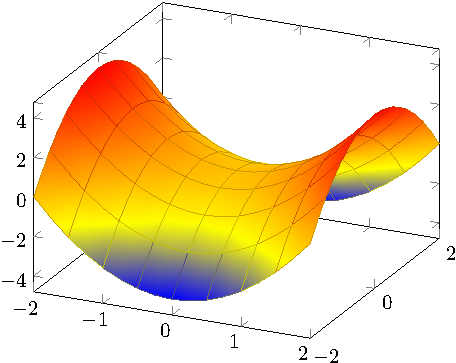
\includegraphics[width=0.75\columnwidth]{Figures/Example.pdf}
                \caption{Example figure (obtained from \textit{PGFPlots - A LaTeX package to create plots}. [Online]. Available: \url{https://pgfplots.sourceforge.net/}).}
                \label{fig:figure}
            \end{figure}

        \subsubsection{Tables}
    
            The \verb*|\captionsetup[table]| command customizes the appearance of the captions for tables in the document. The \verb*|\tabletext{}| is used to add notes to tables easily. Table \ref{tab:table} shows an example table.
            
            \begin{table}[H]
                \centering
                \caption{Small table example.}
    		\label{tab:table}
                \begin{tabular}{cc}
            	\toprule
                    \textbf{Column 1} & \textbf{Column 2} \\
                    \midrule
                    Data 1 & Data 2 \\
                    Data 3 & Data 4 \\
                    \bottomrule
                \end{tabular}
                    
                \tabletext{Note: I'm a table text for additional information.}
                    
            \end{table}

    \subsection{Equation}
    
        Equation \ref{ec:equation} shows an example equation. 
    	\begin{equation} \label{ec:equation}
                \frac{\hbar^2}{2m}\nabla^2\Psi + V(\mathbf{r})\Psi = -i\hbar \frac{\partial\Psi}{\partial t}
    	\end{equation} 
        The \textit{amssymb} package was not necessary to include, because stix2 font incorporates mathematical symbols for writing quality equations. In case you choose another font, uncomment the package in \textit{tau class} code.

        If you want to change the values that adjust the spacing above and below the equations, go to \textit{tau class-math packages} section and play with \verb|\setlength{\eqskip}{8pt}| value until the preferred spacing is set. See appendix for more information.

\section{Environment}

    The \textit{tau class} includes custom environments designed to enhance the presentation of information within documents. Among these custom environments are \textbf{tauenv}, \textbf{info} and \textbf{note} defined in \textit{tauenvs.sty}.

    \begin{tauenv}[frametitle=Custom title]
        This is an example of the custom title environment. To add a title type \verb|[frametitle=Your title]| next to the beginning of the environment (as shown in this example).
    \end{tauenv}

    One of the main features of the info and note environment is that they automatically change the language of their titles (currently English and Spanish) but, you can make a modification in \textit{tauenvs.sty}. See appendix for more information.

\section{Adding codes}

    \textit{Tau class} includes the \textit{listings} package \footnote{Hello there! I am a footnote.}, which offers versatile and customizable features for adding codes in \LaTeX\ documents. Specifically for C, C++, \LaTeX\ and Matlab codes. 

    For C and C++ codes, the \textit{listings} package recognizes the syntax of these programming languages and highlights keywords, comments, and string literals accordingly.

    Similarly, for Matlab codes, the \textit{listings} package offers syntax highlighting and line numbering.
    
    \lstinputlisting[caption=Example of Matlab code., language=Matlab]{example.m}

\section{References}

    The default formatting for references follows the IEEE style. This style is commonly used for technical documents, research papers, and scholarly articles in engineering fields \cite{einstein}.

    At the end of the document, you will find an example of the default reference formatting \cite{dirac}. You can modify the style of your references in the \textit{biblatex} section in \textit{tau.cls}. See appendix for more information.
    
\section{Appendix}

    \subsection{Alternative title}

         You can make the following modification to \textit{tau class} in the \textit{title preferences} section to change the position of the title. This will move the title to the center. 

\begin{lstlisting}[language=TeX, caption=Alternative title.]
\newcommand{\titlepos}{\Centering}
\end{lstlisting}

    \subsection{Equation skip value}

        Play with the value of \verb|\eqskip| until the preferred spacing is set for equations.

\begin{lstlisting}[language=TeX, caption=Equation skip code.]
\newlength{\eqskip}\setlength{\eqskip}{8pt}
\expandafter\def\expandafter\normalsize\expandafter{%
    \normalsize%
    \setlength\abovedisplayskip{\eqskip}%
    \setlength\belowdisplayskip{\eqskip}%
    \setlength\abovedisplayshortskip{\eqskip-\baselineskip}%
    \setlength\belowdisplayshortskip{\eqskip}%
}
\end{lstlisting}

    \subsection{Environments}

        \subsubsection{Environments language}

            The following code defines the language for the environment note

\begin{lstlisting}[language=Tex, caption= Note language.]
\newcommand{\notelanguage}{
    \iflanguage{spanish}{
        {\bfseries\noindent Nota}%
    }{%
        {\bfseries\noindent Note}   % Modify if required in another language
    }%
}
\end{lstlisting}

        and info,

\begin{lstlisting}[language=Tex, caption= Info language.]
\newcommand{\infolanguage}{
    \iflanguage{spanish}{
        {\bfseries\noindent Informaci\'on}%
    }{%
        {\bfseries\noindent Information}    % Modify if required in another language
    }%
}
\end{lstlisting}
		
	\subsubsection{Note}

            This code defines the note environment.

  		\begin{note}
                Lorem ipsum dolor sit amet, consectetur adipiscing elit. Sed vestibulum justo quis massa aliquet, ut ultrices quam bibendum.
		\end{note}
		
\begin{lstlisting}[language=TeX, caption=Note environment code.]
\newmdenv[
	backgroundcolor=taucolor!22, 						
	linecolor=taucolor,									
	linewidth=0.7pt,
	frametitle=\vskip0pt\bfseries\notelanguage,
	frametitlerule=false,
	frametitlefont=\color{taucolor}\bfseries\sffamily,
	frametitlealignment=\raggedright,
	innertopmargin=3pt,
	innerbottommargin=6pt,
	innerleftmargin=6pt,
	innerrightmargin=6pt,
	font=\normalfont,
	fontcolor=taucolor,									
	frametitleaboveskip=3pt,
	skipabove=10pt
]{note} \end{lstlisting}

        \subsubsection{Info}

            This code defines the info environment.

    	\begin{info}
                Lorem ipsum dolor sit amet, consectetur adipiscing elit. Sed vestibulum justo quis massa aliquet, ut ultrices quam bibendum.
		\end{info}
		
\begin{lstlisting}[language=TeX, caption=Info environment code.]
\newmdenv[
	backgroundcolor=taucolor!22, 						
	linecolor=taucolor,									
	linewidth=0.7pt,
	frametitle=\vskip0pt\bfseries\infolanguage,
	frametitlerule=false,
	frametitlefont=\color{taucolor}\bfseries\sffamily,
	frametitlealignment=\raggedright,
	innertopmargin=3pt,
	innerbottommargin=6pt,
	innerleftmargin=6pt,
	innerrightmargin=6pt,
	font=\normalfont,
	fontcolor=taucolor,									
	frametitleaboveskip=3pt,
	skipabove=10pt
]{info} \end{lstlisting}

    \subsection{References}

        This code defines the reference style, you can modify it directly in the \textit{tau.cls-biblatex} section if required.

\begin{lstlisting}[language=TeX, caption=References style.]
\RequirePackage[
    backend=biber,
    style=ieee,
    sorting=ynt
]{biblatex}

\addbibresource{tau.bib}
\end{lstlisting}

\section{Contact me}

    Enjoy writing with tau \LaTeX\ class\hspace{5pt}\faChessKnight \\ 

    \noindent\faWix\hspace{5pt}\href{https://memonotess1.wixsite.com/memonotess}{https://memonotess1.wixsite.com/memonotess} \\
    \faEnvelope[regular]\hspace{5pt}memo.notess1@gmail.com \\
    \faInstagram\hspace{5pt}memo.notess
    
%----------------------------------------------------------

\addcontentsline{toc}{section}{References}
\printbibliography

%----------------------------------------------------------

\end{document}